\paragraph{Tijdsduur}
Net zoals bij native wordt er enkel naar het CPU en geheugen gebruik tijdens 
het afspelen van audio en video gekeken.

\paragraph{CPU \& geheugen}
\begin{figure}[H]
    \centering
    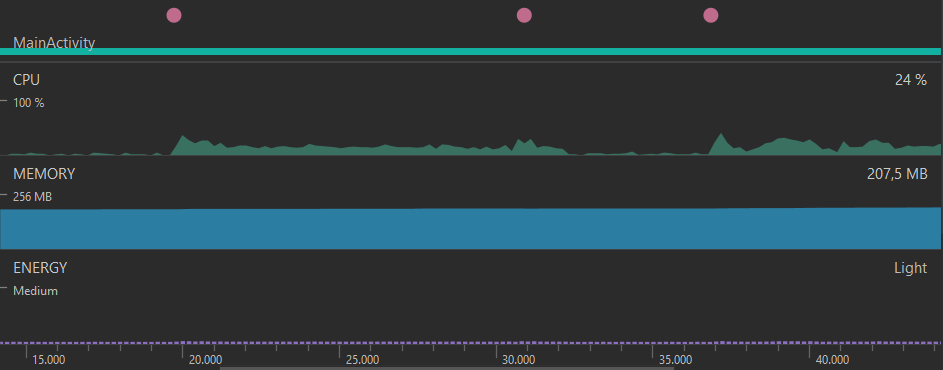
\includegraphics[height=0.25\textheight]{mediaPerformantieCross.png}
    \caption{Overzicht CPU en geheugen gebruik tijdens het afspelen van audio en video bij React Native.}
\end{figure}
Bij het eerste klik event voor het starten van de audio stijgt het
CPU gebruik tot 42\% en zakt daarna af tot een wisselend gebruik van 15 - 25\%. Bij het
tweede klik event voor het pauzeren van de audio stijgt het CPU gebruik tot 35\%. 
Bij het derde klik event voor het starten van de video stijgt het CPU gebruik tot 43\% en 
blijft dan schommelen tussen 10 - 35\%. Tijdens het afspelen van de audio en video blijft 
het geheugen gebruik rond de 207MB hangen. Er is dus geen verschil in
geheugen gebruik bij het afspelen van audio of video en het inactief zijn van de applicatie.
